%
%
%		Finding: Template
%		Author: the DR
%
%
\renewcommand{\FindingAuthor}{Taksh Medhavi}
% DO NOT USE \par, \newline or any other line breaking command in FindingName => report will not build
\renewcommand{\FindingName}{Weak Application Signature}
\renewcommand{\Location}{dummyapplication.apk}
\renewcommand{\Component}{META-INF/CERT.SF}
\renewcommand{\FoundWith}{TODOTODO}
\renewcommand{\TestMethod}{TODOTODO}
\renewcommand{\CVSS}{4.7}
\renewcommand{\CVSSvector}{CVSS:3.1/AV:L/AC:H/PR:L/UI:N/S:U/C:N/I:H/A:N}
\renewcommand{\CWE}{328}
% Poor-man's combo boxes:
% High, Medium, Low, Info, TBR (To Be Rated)
\renewcommand{\Criticality}{Medium}
% Easy, Average, Hard, TBR (To Be Rated)
\renewcommand{\Exploitability}{Hard}
% Access control, Application Design, Information Disclosure, Outdated Software, Security Configuration
\renewcommand{\Category}{Undefined}
% Easy, Average, Difficult, TBR (To Be Rated)
\renewcommand{\Detectability}{Easy}


\ReportFindingHeader{\FindingName}


%-------------------------------------------
%	Details                                |
%-------------------------------------------

\subsection*{Details}

Application uses SHA1 for application signing. Also, application supports Android v1 signing. For Android 5.0 to 8.1, it can lead to Janus vulnerability. Currently application is supporting Android 5.0 and higher versions.


%-<Details>
%-------------------------------------------
%	Impact                                 |
%-------------------------------------------



\subsection*{Impact}

SHA1 has flaws with regards to collisions and it is considered weak hashing algorithm. In Janus vulnerability scenario, the attacker can modify the code in applications without affecting their signatures.

% \emph{TODOTODO}.

%-<Impact>
%-------------------------------------------
%	Repeatability                          |
%-------------------------------------------

\newpage


\subsection*{Repeatability}

Application is using deprecated SHA1 algorithm and supports v1 also as shown in \cref{figure:APK_sign}. 

\begin{figure}[H]
\centering
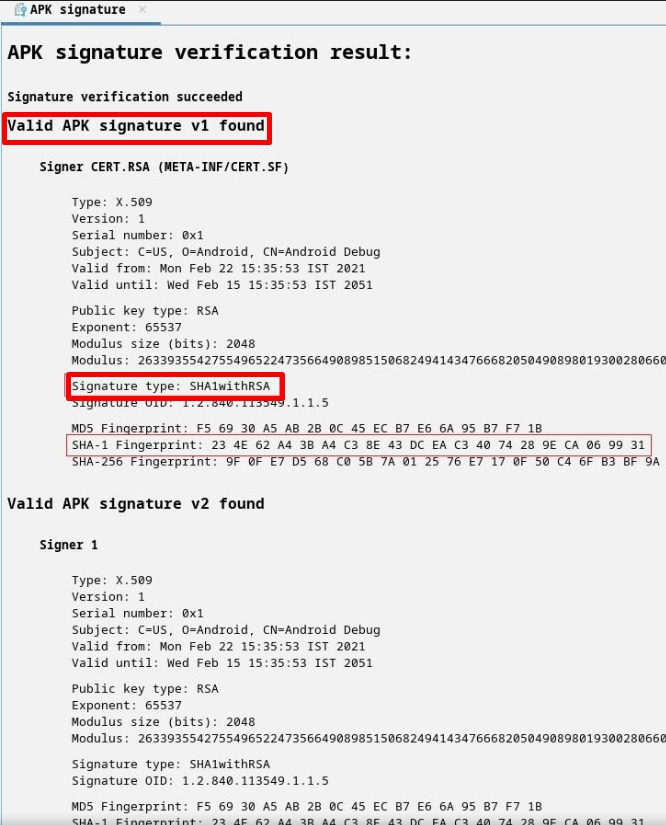
\includegraphics[scale=0.9,frame]{\CurrentFilePath/APK_sign}
\caption{Application signed with v1}
\label{figure:APK_sign}
\end{figure}

\pagebreak
Application also supports Android minimum SDK version 21 which allows application to be installed on devices with Android 5.0 and higher.
\begin{figure}[H]
\centering
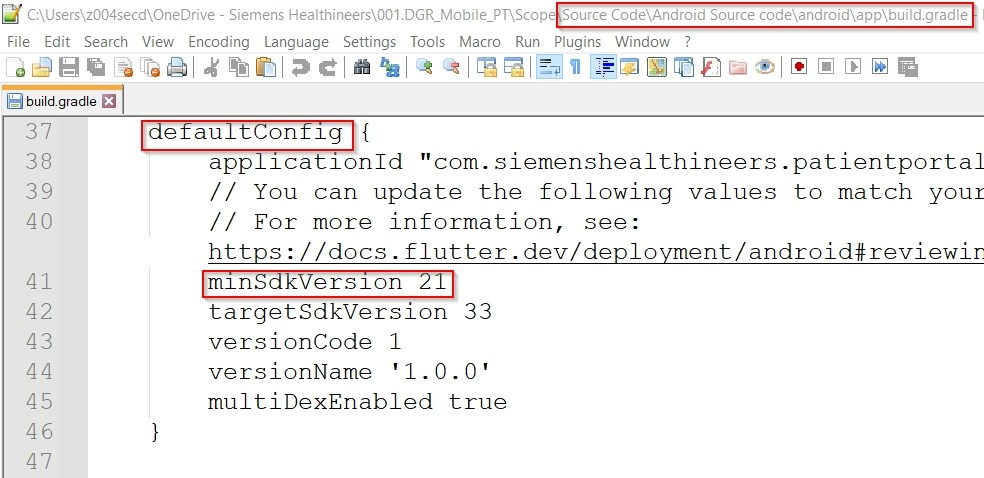
\includegraphics[scale=0.6,frame]{\CurrentFilePath/gradle_file}
\caption{Application supports minSdkVersion 21}
\label{figure:gradle_file}
\end{figure}


%-<Repeatability>
%-------------------------------------------
%	Countermeasures                        |
%-------------------------------------------



\subsection*{Countermeasures}

Sign the application with v2 signature with SHA256 hash. For Android device below version 8.0, Janus vulnerability is applicable for all versions of signature, so application should support Android device above 8.0 to avoid it. It can be achieved by changing default configuration value of "minSdkVersion" parameter in build.gradle file.

%-<Countermeasures>
%-------------------------------------------
%	References - pulls bib entries         |
%-------------------------------------------



\subsection*{References}

This finding references the following information sources:

\begin{itemize}
	\item \href{https://www.first.org/cvss/calculator/3.1#CVSS:3.1/AV:L/AC:H/PR:L/UI:N/S:U/C:N/I:H/A:N}
	{CVSS 4.7}
	\item \href{https://nvd.nist.gov/vuln/detail/CVE-2017-13156}
	{Janus Vulnerability: CVE-2017-13156}
	\item \bibentry{CWE-328}
\end{itemize}


%-<References>


